\section{Grundlagen Elektrotechnik}

\subsection{Ladung}
Wichtigster Grundsatz: \textbf{Ladung ist eine Eigenschaft}.\\
Jedes Elementarteilchen hat eine Elementarladung. 
Daher ist jede gemessene Ladung immer ein vielfache, dieser Elementarladung.\\
Die wichtigsten Eigenschaften sind:
\begin{itemize}
    \item Es gibt 2 Arten. Positiv und negativ
    \item Gleiche Ladung stossen sich ab, ungleiche ziehen sich an
    \item Ladung ist quantisierbar (ein Vielfaches einer Elementarladung)
    \item Ladung bleibt insgesamt erhalten
    \item Ladung ist an Masse gebunden
\end{itemize}
Ladung wird in \unit{\coulomb}  $\widehat{=}$ \unit{\ampere\second} quantisiert.

\subsection{Ladungstransport}

Elektrische Ladung wird unterschiedlich gut in verschiedenen Medien transportiert.\\

\begin{center}
    \begin{tabular}{|l|l|l|} \hline  
        \textbf{Medium} & \textbf{Beweglicher Ladungsträger} & \textbf{Beispiele}\\ \hline\hline 
            Metalle & freie Elektronen & Cu, Ag, Au,.... \\\hline
            Elektrolyte& freie Ionen&Salzwasser, Säuren, Laugen, ....\\\hline
            Gase, Plasma& freie Elektronen, freie Ionen&FL-Röhren, Sonnenplasma\\\hline
            Halbleiter& Freie Elektronen, Löcher&Si, Ge, Se, GaN, ...\\\hline
            Vakuum& Keine(\say{nichts})&CRT-Bildschirme\\\hline
            Isolatoren& \say{nichts}&Keramik, Kunststoffe, ...\\\hline
    \end{tabular}
\end{center}

Luft kann dabei zu den Gasen und zu den Isolatoren gezählt werden, je nach Spannung welche herrscht.\\

\subsection{Elektrischer Strom}

Elektrischer Strom ist der Transport von Ladung.
\[ \text{Einfache definition: I} = \dfrac{\Delta\text{Q}}{\Delta\textbf{t}} = \dfrac{\text{N}_\text{e}}{\Delta\textbf{t}}\]
\[\text{Masseinheit: }[\text{I}] = \dfrac{[\text{Q}]}{[\text{t}]} = \dfrac{\unit{\ampere\second}}{\unit{\second}} = \dfrac{\unit{\coulomb}}{\unit{\second}} = \unit{\ampere}\]
Elektrischer Strom braucht immer eine Bezugsrichtung:\\
\begin{wrapfigure}{l}{0.3\linewidth}
    \includesvg[width = \linewidth, inkscapelatex=false]{svg/Elektrischer Strom.svg}
\end{wrapfigure}
Die Richtung des elektrischen Stromes sagt aus in welche Richtung sich die Elektronen bewegen. 
Es wird zwischen der technischen und der physikalischen Richtung unterschieden, welche entgegen einander verlaufen. 
Die Elementarladung eines Elektrons ist negativ.\\

\subsection{Stomdichte(rechtwinklig zur Fläche)}

Stomdichte sagt aus wie viel Strom über einen Querschnitt fliesst. 
In einem Leiter ohne konstanten Querschnitt bleibt die Stromdichte proportional zur Fläche.
\[\text{Masseinheit: }[\text{J}] = \dfrac{[\text{I}]}{[\text{A}]} = \dfrac{\unit{\ampere}}{\unit{\square\meter}}\]\\


\begin{center}
    \includesvg[width = 0.8\linewidth, inkscapelatex=false]{svg/Stromdichte.svg}
\end{center}

\subsubsection{Schmelzstromdichte}

Die Schmelzstromdichte sagt aus wie viel Strom durch einen Leiter fliessen muss bis dieser anfängt zu schmelzen (typischerweise tausende \unit{\ampere}).

\subsection{Elektrisches Potenzial}

Elektrisches Potenzial ist Arbeit, die für den Spannungstransport zur Verfügung steht oder die Freigesetzt wird bei Transport der Ladung. 

\[ \text{Einfache Definition:} [\varphi] = \frac{\Delta[\text{W}]}{[\text{Q}]} = \frac{\text{J}}{\text{C}} = \unit{\volt} = \frac{\unit{\square\meter\kilo\gram}}{\unit{\cubic\second\ampere}}\]

\subsection{Elektrische Spannung}

Elektrische Spannung ist ein Potenzialunterschied. 
Dh. Elektrische Spannung ist eine Differenz von Energie, die zum Ladungstransport zur Verfügung steht.

\[ \text{Einfache Definition :}[\text{U}] = \varphi_a - \varphi_b = \unit{\volt}   \]

\subsection{Kirchhoff current law / Kirchhoff 1 / KCL}

Das Kirchhoff current law sagt aus das die Summe aller Ströme in einem geschlossenen Knoten 0 sein müssen.

\[ \sum_{n} \text{I}_n = 0\]

Die einzige Bedingung ist das alle Ströme dieselbe Bezugsrichtung haben.

\begin{center}
    % LTeX: enabled=false
\begin{tikzpicture}
    % Define the style for the currents
    \tikzset{current/.style={-{Latex[length=2.5mm]},thick}}
  
    % Draw the node for the junction
    \node[draw, circle, minimum size=0.3cm] (Junction) at (0,0) {};
  
    % Draw the currents entering and leaving the junction
    \draw[current] (-2,0) -- (Junction) node[midway, above] {\(I_2\)};
    \draw[current] (Junction) -- (2,0) node[midway, above] {\(I_1\)};
    \draw[current] (0,-2) -- (Junction) node[midway, right] {\(I_3\)};
  
    % Optionally, add plus and minus signs
    \node at (-0.7,0.3) {+};
    \node at (1.4,0.3) {-};
    \node at (0.5,-1) {+};
  \end{tikzpicture}
\end{center}

\subsection{Kirchhoff voltage law / Kirchhoff 2 / KCV}

Die Summe aller Teilspannungen in einer Masche ist 0. 

\[ \sum_{n} \text{U}_n = 0\]

Die Bedingung ist das alle Spannungen dasselbe Referenzpotential haben.

\subsection{Elektrische Leistung}

Elektrische Leistung ist Arbeit pro Zeit.

\[ \text{Definition :} [\text{P}] = \frac{\Delta[\text{W}]}{\Delta[\text{t}]} = \frac{\unit{\joule}}{\unit{\second}} = \frac{\unit{\volt\ampere\second}}{\unit{\second}} = \unit{\volt\ampere} = \unit{\watt} \]

\subsection{Verbraucher oder Quelle} \label{source_sink}

Um ein Verbraucher und eine Quelle auseinander zu halten kann man sich die Richtungen der Spannung und des Stromes überprüfen. Ist die Spannung  und der der Strom parallel zu einander, handelt es sich um ein Verbraucher(Wie ein Widerstand). Ist die Spannung und der Strom antiparalell, handelt es sich um eine Quelle (aus einer Spannungsquelle fliesst ein Strom hinaus).\\

\begin{center}
    % LTeX: enabled=false
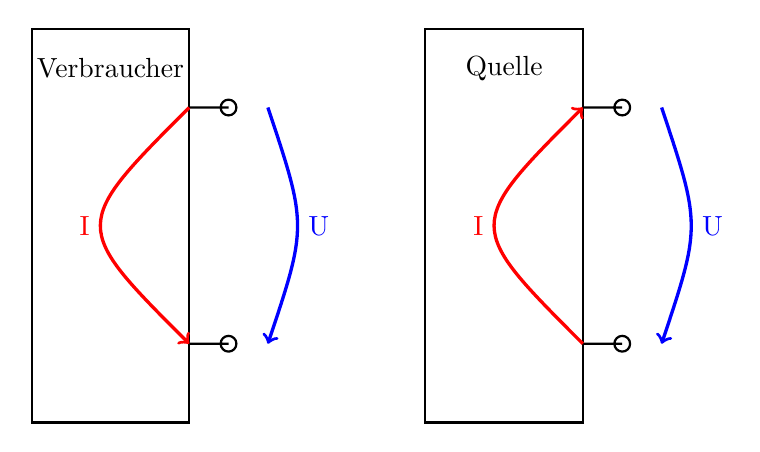
\begin{tikzpicture}
    \draw[thick] (0,0) rectangle (2,5);
    \node at (1,4.5) {Verbraucher};
    \foreach \y in {1,4}
        \draw[thick] (2,\y) -- ++(0.5,0) circle [radius=0.1];

    \draw[<-,red,very thick] (2,1) .. controls (0.5,2.5) .. (2,4) node[midway,left] {I};
    \draw[<-,blue,very thick] (3,1) .. controls (3.5,2.5) .. (3,4) node[midway,right] {U};

    \draw[thick] (5,0) rectangle (7,5);
    \node at (6,4.5) {Quelle};
    \foreach \y in {1,4}
        \draw[thick] (7,\y) -- ++(0.5,0) circle [radius=0.1];

    \draw[->,red,very thick] (7,1) .. controls (5.5,2.5) .. (7,4) node[midway,left] {I};
    \draw[<-,blue,very thick] (8,1) .. controls (8.5,2.5) .. (8,4) node[midway,right] {U};      
\end{tikzpicture}  

\end{center}    

\subsection{Elektrischer Widerstand / Leitwert}

Elektrischer Widerstand / Leitwert ist eine Konsequenz des Zusammenhangs von Elektrischen Strom und Spannung. 
\[\text{I}   \underbrace{\text{ist Proportional zu}}_\propto{}   \text{U} \\ \text{I} = \text{G}\cdot\text{U}\]\\
G ist der so genannte Elektrische Leitwert und von oben abgeleitet: $\text{G} = \dfrac{\text{I}}{\text{U}}$ in der Masseinheit \unit{\siemens}(Siemens).\\
Der Elektrische Widerstand entsteht durch den Kehrwert von dem Leitwert $[\text{R}] = \dfrac{1}{[\text{G}]} = \dfrac{\text{[\text{U}]}}{[\text{I}]} = \unit{\ohm} $ (Ohm).\\

\subsection{Leitfähigkeit}

Elektrische Leitfähigkeit ist eine Materialeigenschaft und hängt von der Mobilität, Anzahl freier Ladungsträger und der Ladung der freien Ladungsträger ab.\\
\begin{align*}
    [\text{Leitfähigkeit}]& = \text{n}\cdot\text{q}\cdot\text{\textmu} = \sigma = \unit[per-mode=fraction]{\ampere\per\volt\per\meter} = \unit[per-mode=fraction]{\siemens\per\meter}\\
    \text{n}& = \text{Anzahl freier Ladungsträger}\\
    \text{q}& = \text{Ladung pro Ladungsträger}\\
    \text{\textmu}& = \text{Mobilität / Freiheit der Elektronen sich zu bewegen}\\
\end{align*}


Die Faktoren \say{n} und \say{q} sind dabei Material konstanten. 
Die Variable \say{\textmu} ist allerdings temperaturabhängig. 

\subsubsection{Mobilität}

Die Mobilität (\textmu) eines Ladungsträgers setzt sich wie folgt zusammen:
\begin{align*}
    \text{\textmu}& =  \frac{\text{q}\tau}{\text{m}}\\
    \text{q}& = \text{Ladung des Ladungsträger}\\
    \tau& = \text{Mittlere Stoszeit zwischen den Ladungsträger}\\
    \text{m}& = \text{Masse des Ladungsträger}\\
    \newline
    [\text{\textmu}]& = \unit[per-mode=fraction]{\coulomb\second\per\kilo\gram} = \unit[per-mode=fraction]{\square\meter\per\volt\per\second}
\end{align*}


\subsubsection{Spezifischer Widerstand}

Der Kehrwert der Leitfähigkeit wird oftmals auch verwendet:\\

\[ [\text{Spezifischer Widerstand}] = \left[ \frac{1}{\sigma} \right] = [\varrho] = \unit[per-mode=fraction]{\volt\per\meter\per\ampere}\]

\subsubsection{Widerstandsberechnungen}

Um aus Leitfähigkeit und spez. Widerstand einen Widerstand berechnen zu können können folgende Formeln verwendet werden.\\
\[
\unit{\ohm} = \frac{\varrho\cdot[\text{Leiterlänge}]}{[\text{Leiterfläche}]} = \frac{\varrho \cdot \unit{\meter}}{\unit{\square\meter}}\\
\unit{\ohm} = \frac{[\text{Leiterlänge}]}{\sigma\cdot[\text{Leiterfläche}]} = \frac{\unit{\meter}}{\sigma\cdot\unit{\square\meter}}\\
\]

Allerdings sind diese Formeln nicht allgemeingültig und können nur dann verwendet werden, wenn die Feldlinien senkrecht zu der Fläche stehen(und sich das nicht verändert). 
Manchmal wird die Einheit auch gekürzt dargestellt (machen aber nur evtl fiese Dozenten).

\subsection{Temperaturabhängigkeit}

Nicht ideale Widerstände ändern ihren Wert, unter anderem, abhängig mit der Temperatur. 
In der Regel ändern sich der Widerstand nicht linear und ist von Widerstand zu Widerstand etwas anders. 
Um trotzdem Widerstandswerte annähern zu können wird die Funktion des Widerstands angenähert. 
Dies erfolgt je nach Anwendung mit einem, zwei oder noch mehr Termen.
\[
\begin{aligned}
    \Delta\text{T}& = \alpha\cdot\Delta\text{T}\cdot\text{R}_\text{t20} &\rightarrow \text{Lineare Annäherung}\\
    \Delta\text{T}& = (\alpha\cdot\Delta\text{T} + \beta\cdot\Delta\text{T})\cdot\text{R}_\text{t20} &\rightarrow \text{Quadratische Annäherung}\\
    &\text{ ...}\\
    \text{R}_{(\text{T})}& = (1 + \alpha\cdot\Delta\text{T})\cdot\text{R}_\text{t20} &\rightarrow \text{Lineare Annäherung}\\
    \text{R}_{(\text{T})}& = (1 + \alpha\cdot\Delta\text{T} + \beta\cdot\Delta\text{T})\cdot\text{R}_\text{t20} &\rightarrow \text{Quadratische Annäherung}\\
\end{aligned}
\]

Der Widerstand $\text{R}_\text{t20}$ setzt hier jeweils den \say{Nullpunkt} oder den Ausgangspunkt, von welcher aus die Temperatur berechnet wird.

\subsubsection{PPM's}

Eine andere, in der Praxis häufig verwendete Art, Temperaturkoeffizienten anzugeben, sind die so genannten PPM's oder auch parts per milion (in der Praxis auch TCR / temperature coefficient). 
Diese sagen aus um wie viel sich ein Widerstands Wert pro Grad Kelvin ändert daher handelt es sich hier nur um ein lineares Modell mit beschränkter Genauigkeit. 
Sie haben meist keine Potenz oder sind ganzzahlig da, wie der Name es schon andeutet, sie mit $10^{-6}$ multipliziert werden. 
Die korespondierende Formel dazu lautet:\\
\[
    \frac{\Delta\text{R}(\Delta\text{T})}{\text{R}_{\text{T0}}} = \frac{\Delta\text{R}}{10^{6}}
\]
